\section{Riverbed}

\subsection{Motivation}
In a web service, a client like a desktop
browser or a smartphone app interacts with datacenter
machines. Although smartphones and web browsers provide
rich platforms for computation, the core application
state typically resides in cloud storage. This state
accrues much of its value from server-side
computations that involve no participation (or explicit
consent) from end-user devices.

By running the bulk of an application within VMs
in a commodity cloud, developers receive two
benefits. First, developers shift the burden of server
administration to professional datacenter operators. Second,
developers gain access to scale-out resources that vastly
exceed those that are available to a single user device.
Scale-out storage allows developers to co-locate large
amounts of data from multiple users; scale-out computation
allows developers to process the co-located data for the
benefit of users (e.g., by providing tailored search
results) and the benefit of the application (e.g., by
providing targeted advertising).

\paragraph{A Loss of User Control:}
Unfortunately, there is a disadvantage to migrating
application code and user data from a user's local
machine to a remote datacenter server: the user
loses control over where her data is stored, how it is
computed upon, and how the data (and its derivatives)
are shared with other services. Users are increasingly
aware of the risks associated with unauthorized data
leakage~\cite{badCharities,whatsappSued,ashleyMadison},
%and proposals like the ``Do Not Track'' HTTP header~\cite{}
%and the ``right to be forgotten'' by search engines~\cite{}
%represent attempts to restore some of the data control
%that users have lost.
and some governments have begun to mandate that online
services provide users with more control over how their
data is used. For example, in 2016, the EU passed the
General Data Protection Regulation~\cite{gdpr}.
Articles~6, 7, and 8 of the GDPR state that users
must give consent for their data to be accessed.
Article 15 establishes a ``right to access,'' mandating
that users have the ability to know how their data
is being processed by a company. Article 17 defines
a user's right to request her data to be deleted;
Article 32 requires a company to implement ``appropriate''
security measures for data-handling pipelines.
Unfortunately, requirements like these \textit{lack
	strong definitions and enforcement mechanisms at the systems
	level.} Laws like GDPR provide little technical guidance
to a developer who wants to comply with the laws while
still providing the sophisticated applications that
users enjoy.
%For example, web services are free to ignore ``Do Not Track''
%requests, and commodity frameworks for large-scale data processing
%offer no facilities for expressing or enforcing user-centric
%data policies like the right to be forgotten.

The research community has proposed information flow control
(IFC) as a way to constrain how sensitive data spreads
throughout a complex system~\cite{hedin11,li03}. IFC assigns
labels to program variables or OS-level resources like
processes and pipes; given a partial ordering which defines
the desired security relationships between labels, an IFC
system can enforce rich properties involving data secrecy
and integrity. Unfortunately, traditional IFC is too burdensome
to use in modern, large-scale web services. Creating and
maintaining a partial ordering of labels is too difficult---the
average programmer or end-user struggles to reason about data
safety using the abstraction of fine-grained label hierarchies.
As a result, no popular, large-scale web service uses IFC to
restrict how sensitive data is processed and shared.

\begin{figure}[t!]
	\centering
	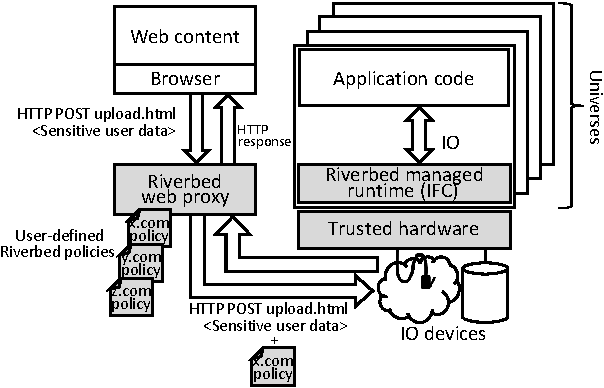
\includegraphics[width=0.48\textwidth]{riverbed-overview.pdf}
	\vspace{-5mm}
	\caption{Riverbed's architecture. The user's
		client device is on the left, and the
		web service is on the right. Unmodified components
		are white; modified or new components are grey.}
	\label{fig:arch}
\end{figure}

\subsection{Riverbed Overview}
In this thesis, we introduce Riverbed, a distributed web platform
for safeguarding the privacy of user data. Riverbed provides
benefits to both web developers and to end users. To web
developers, Riverbed provides a \emph{practical} IFC system
which allows developers to easily ``bolt on'' stronger security
policies for complex applications written in standard managed
languages. To end users, Riverbed provides a straightforward
mechanism to verify that server-side code is running within a
privacy-preserving environment.

Figure~\ref{fig:arch} describes Riverbed's architecture. For each
Riverbed web service, a user defines an information flow policy
using simple, human-understandable constraints like ``do not
save my data to persistent storage'' or ``my data may only be
sent over the network to \texttt{foo.com}.'' In the common case,
users employ predefined, templated policy files that are designed
by user advocacy groups like the EFF. When the user generates
an HTTP request, a web proxy on the user's device transparently
adds the appropriate data flow policy as a special HTTP header. 

Within a datacenter, Riverbed leverages the fact that many
services run atop managed runtimes like Python, .NET, or
the JVM. Riverbed modifies such a runtime to automatically
taint incoming HTTP data with the associated user policies.
As the application derives new data from tainted bytes,
the runtime ensures that the new data is also marked as
tainted. The runtime ensures that, whenever an application
tries to externalize data via the disk or the network, the
externalization is only allowed if it is permitted by user
policies. An application process which attempts a disallowed
externalization is automatically terminated.

In Riverbed, application code (i.e., the code which the
managed runtime executes) is totally unaware that IFC
is occurring. Indeed, application developers have no way
to read, write, create, or destroy taints and data flow
policies. The advantage of this scheme is that it makes
Riverbed compatible with code that has not been explicitly
annotated with traditional IFC labels. However, different
end users will likely define incompatible data flow policies.
As a result, policy-agnostic code would quickly generate a
policy violation for some subset of users; Riverbed would
then terminate the application. To avoid this problem,
Riverbed spawns multiple, lightweight copies of the service,
one for each set of users who share the same data flow policies.
We call each copy a \textit{universe}. Since users in the
same universe allow the same types of data manipulations,
any policy violations indicate true problems with the
application (e.g., the application tried to send sensitive
data to a server that was not whitelisted by the inhabitants
of the universe). Developers can then fix these violations
to ensure that code respects the desired privacy protections
for the target user demographic.

Before a user's Riverbed proxy sends data to a server, the
proxy employs remote software attestation~\cite{remoteAttestation}
to verify that the server is running an IFC-enforcing Riverbed
runtime. Importantly, a trusted server will perform \textit{next-hop
	attestation}---the server will not transmit user data to
another network endpoint unless that endpoint is an
attested Riverbed runtime whose TLS certificate name is
explicitly whitelisted by the user's data flow policy.
In this manner, Riverbed enables controlled data sharing
between machines that belong to different services.

\subsection{Our Contributions}
To the best of our knowledge, Riverbed is the first distributed
IFC framework which is practical enough to support large-scale,
feature-rich web services that are written in general-purpose
managed languages. Riverbed preserves the traditional advantages
of cloud-based applications, allowing developers to offload
administrative tasks and leverage scale-out resources. However,
Riverbed's universe mechanism, coupled with a simple policy language,
provides users with understandable, enforceable abstractions
for controlling how datacenters manipulate sensitive data.
Riverbed makes it easier for developers to comply with laws like
GDPR---users give explicit consent for data access via Riverbed
policies, with server-side universes constraining how
user data may be processed, and where its derivatives can
be stored.

We have ported several non-trivial applications to Riverbed,
and written data flow policies for those applications. Our
experiments shows that Riverbed enforces data flow policies
with worst-case end-to-end overheads of 10\%; Riverbed also
supports legacy code with little or no developer intervention,
making it easy for well-intentioned (but average-skill)
developers to write services that respect user privacy.

\subsection{Threat Model}

Riverbed assumes that developers want to enforce user-defined
privacy policies, but are loathe to refactor code to do so.
Thus, Riverbed assumes that server-side code is weakly adversarial:
poorly-designed applications may unintentionally try to leak
data via explicit flows, but developers will not intentionally
write code that attempts to surreptitiously leak data, e.g.,
via implicit flows, or via targeted attacks on the taint-tracking
managed runtime.

A datacenter operator has physical access to servers, which
enables direct manipulation of server RAM. So, our current
Riverbed prototype assumes that datacenter operators are trusted. 
To ease this assumption, Riverbed could leverage a hardware-enforced
isolation mechanism like Intel SGX~\cite{sgx}. SGX allows a
secure computation to execute on a private core, with the
hardware automatically encrypting and hashing the content
of memory writes so that other cores are unable to inspect or
modify the RAM that belongs to the secure computation.
Ryoan~\cite{ryoan} creates a distributed sandbox by representing
an application as a directed graph of SGX computations that
run on different servers. Unfortunately, SGX places limits on
the memory size of secure applications. SGX also requires
the applications to run in ring 3, forcing the code to rely
on an untrusted OS in ring 0 to perform IO; the result is a
large number of context switches for applications that perform
many IOs~\cite{haven}. Riverbed strives to be compatible with
complex applications that often perform IO. So, Riverbed eschews
mechanisms like SGX, and must be content to not protect against
actively-malicious datacenter operators.
% Note that SGX does allow an enclave's code to be
% multithreaded and run on multiple cores: see Section 5.2.4 of https://eprint.iacr.org/2016/086.pdf
To implement remote attestation, Riverbed does rely
on trusted server-side TPM hardware,
but TPMs do not protect against physical attacks on
the main server hardware.

Riverbed assumes that the entire client-side is trusted,
with the exception of the web content in a particular
page. Buggy or malicious content may try to disclose
too much information to a server. However, Riverbed
ensures that whatever data is sent will be properly tagged.
Since Riverbed uses TLS to authenticate network endpoints,
the HTTPS certificate infrastructure must be trusted.

On the server, Riverbed's TCB consists of the taint-tracking
managed runtime, a reverse proxy that forwards requests to
the appropriate universes, the TPM
hardware~\cite{tpmchip} that provides the root of trust for attestation,
and the daemon which servers use to attest to clients. We make
standard cryptographic assumptions about the strength of the
ciphers and hash functions used by the attestation protocol.
Between the trusted hardware and the managed runtime are a boot
loader, an OS, and possibly other systems software. Each end-user
can select a different set of systems software to trust. These
selections reside within the user's policies,
so that Riverbed's client-side proxy can refuse to disclose data
to untrusted server-side systems code.
